\documentclass[11pt]{article}

\newcommand{\titrechapitre}{Suites arithmétiques et géométriques -- Exercices}
\newcommand{\titreclasse}{Lycée Jean-Baptiste \textsc{Corot}}
\newcommand{\pagination}{\thepage}%{\thepage/\pageref{LastPage}}
\newcommand{\topbotmargins}{2cm}
%%%%%%%%%%%%%%%%%%%%%%%%%%%%%%%%%%%%%%%%%%%%%%%%%%%%%%%%%%%%%%%%%%%%%%%%%%%%%%%%
%
% PACKAGES
% ========
%
%%%%%%%%%%%%%%%%%%%%%%%%%%%%%%%%%%%%%%%%%%%%%%%%%%%%%%%%%%%%%%%%%%%%%%%%%%%%%%%%

\usepackage[english, french]{babel}
\usepackage[utf8]{inputenc}
\usepackage[T1]{fontenc}
\usepackage{graphicx}
\usepackage{amsmath,amssymb,amsthm,amsopn}
\usepackage{hyperref}

% Pour avoir l'écriture \mathscr (math script)
% ============================================

\usepackage{mathrsfs}

% Deal with coma as a decimal separator
% =====================================

\usepackage{icomma}

% Package Geometry
% ================

\usepackage[a4paper, lmargin=2cm, rmargin=2cm, top=\topbotmargins, bottom=\topbotmargins]{geometry}

% Package multicol
% ================

\usepackage{multicol}

% Redefine abstract
% =================

% Note
% ====
%
% Le reste a été commenté pour ne pas charger trop de choses au démarrage. On
% verra si on en a besoin plus tard.
%
% --------
%
%\usepackage{mathrsfs}
%\usepackage{multirow}
%\usepackage{bm}
%\hypersetup{
%    colorlinks=true,
%    linkcolor=blue,
%    citecolor=red,
%}
%\usepackage{diagbox}
%
%\usepackage{algorithm}
%\usepackage{algpseudocode}
%
%\renewcommand{\algorithmicrequire}{\textbf{Input:}}
%\renewcommand{\algorithmicensure}{\textbf{Output:}}


%%%%%%%%%%%%%%%%%%%%%%%%%%%%%%%%%%%%%%%%%%%%%%%%%%%%%%%%%%%%%%%%%%%%%%%%%%%%%%%%
%
% TIKZ
% ====
%
%%%%%%%%%%%%%%%%%%%%%%%%%%%%%%%%%%%%%%%%%%%%%%%%%%%%%%%%%%%%%%%%%%%%%%%%%%%%%%%%

\usepackage{tikz}
\usetikzlibrary{arrows}

\usepackage{tkz-tab} % Variation tables

\usepackage{pgfplots}
%\usepackage{pgf-pie} % Pie charts

\pgfplotsset{
%\newcommand{\settingsgraph}{
x=.5cm,y=.5cm,
xticklabel style = {font=\scriptsize, yshift=.1cm},
yticklabel style = {font=\scriptsize, xshift=.1cm},
axis lines=middle,
ymajorgrids=true,
xmajorgrids=true,
major grid style = {color=white!80!blue},
xmin=-5.5,
xmax=5.5,
ymin=-5.5,
ymax=5.5,
xtick={-5.0,-4.0,...,5.0},
ytick={-5.0,-4.0,...,5.0},
}

% Tikz style

\tikzset{round/.style={circle, draw=black, very thick, scale = 0.7}}
\tikzset{arrow/.style={->, >=latex}}
\tikzset{dashed-arrow/.style={->, >=latex, dashed}}

\newcommand{\point}[3]{\draw[very thick, #3] (#1-.1, #2)--(#1+.1, #2)
(#1, #2-.1)--(#1, #2+.1)}

%%%%%%%%%%%%%%%%%%%%%%%%%%%%%%%%%%%%%%%%%%%%%%%%%%%%%%%%%%%%%%%%%%%%%%%%%%%%%%%%
%
% FANCY HEADER
% ============
%
%%%%%%%%%%%%%%%%%%%%%%%%%%%%%%%%%%%%%%%%%%%%%%%%%%%%%%%%%%%%%%%%%%%%%%%%%%%%%%%%


\usepackage{fancyhdr}
\usepackage{lastpage}

\pagestyle{fancy}
\newcommand{\changefont}{\fontsize{9}{9}\selectfont}
\renewcommand{\headrulewidth}{0mm}
\renewcommand{\footrulewidth}{0mm}

\fancyhead[C]{}
\fancyhead[L]{\titreclasse}
\fancyhead[R]{\titrechapitre}
\fancyfoot[C]{}
\fancyfoot[L]{}
\fancyfoot[R]{\pagination}
\addtolength{\skip\footins}{20pt} % distance between text and footnotes

%%%%%%%%%%%%%%%%%%%%%%%%%%%%%%%%%%%%%%%%%%%%%%%%%%%%%%%%%%%%%%%%%%%%%%%%%%%%%%%%
%
% THEOREM STYLE
% =============
%
%%%%%%%%%%%%%%%%%%%%%%%%%%%%%%%%%%%%%%%%%%%%%%%%%%%%%%%%%%%%%%%%%%%%%%%%%%%%%%%%

\usepackage[tikz]{bclogo}
\usepackage{mdframed}

\usepackage{tcolorbox}
\tcbuselibrary{listings, breakable, theorems, skins}

%\newtheoremstyle{break}%
%{}{}%
%{\itshape}{}%
%{\bfseries}{}%  % Note that final punctuation is omitted.
%{\newline}{}

\newtheoremstyle{scbf}%
{}{}%
{}{}%
%{\scshape}{}%  % Note that final punctuation is omitted.
{\bfseries\scshape}{}%  % Note that final punctuation is omitted.
{\newline}{}

%\theoremstyle{break}
%\theoremstyle{plain}
%\newtheorem{thm}{Theorem}[section]
%\newtheorem{lm}[thm]{Lemma}
%\newtheorem{prop}[thm]{Proposition}
%\newtheorem{cor}[thm]{Corollary}

%\theoremstyle{scbf}
%\newtheorem{exo}{$\star$ Exercice}

%\theoremstyle{definition}
%\newtheorem{defi}[thm]{Definition}
%\newtheorem{ex}[thm]{Example}

%\theoremstyle{remark}
%\newtheorem{rem}[thm]{Remark}

% Defining the Remark environment
% ===============================

\newenvironment{rmq}
  {
    \begin{bclogo}[logo=\bcinfo, noborder=true]{Remarque}
  }
  {
    \end{bclogo}
  }

% Defining the exercise environment
% =================================

\newcounter{exos}
\setcounter{exos}{1}

\newenvironment{exo}
  {
    \begin{bclogo}[logo=\bccrayon, noborder=true]{Exercice \theexos}
  }
  {
    \end{bclogo}
    \addtocounter{exos}{1}
  }


% Redefining the proof environment from amsthm
% ============================================

\tcolorboxenvironment{proof}{
  blanker, breakable, before skip=10pt,after skip=10pt,
  borderline west={1mm}{0pt}{red},
  left=5mm,
}

% Defining the definition environment
% ===================================

\colorlet{coldef}{black!50!green}

\newcounter{defis}
\setcounter{defis}{1}

\newenvironment{defi}[1]
  {
    \begin{defihid}{{#1}}{\thedefis}
  }
  {
    \end{defihid}
    \addtocounter{defis}{1}
  }

\newtcolorbox{defihid}[2]{%
  empty,title={ {\bfseries Définition {#2}} ({#1})},attach boxed title to top left,
boxed title style={empty,size=minimal,toprule=2pt,top=4pt,
overlay={\draw[coldef,line width=2pt]
([yshift=-1pt]frame.north west)--([yshift=-1pt]frame.north east);}},
coltitle=coldef,
before=\par\medskip\noindent,parbox=false,boxsep=0pt,left=0pt,right=3mm,top=4pt,
breakable,pad at break*=0mm,vfill before first,
overlay unbroken={\draw[coldef,line width=1pt]
([yshift=-1pt]title.north east)--([xshift=-0.5pt,yshift=-1pt]title.north-|frame.east)
--([xshift=-0.5pt]frame.south east)--(frame.south west); },
overlay first={\draw[coldef,line width=1pt]
([yshift=-1pt]title.north east)--([xshift=-0.5pt,yshift=-1pt]title.north-|frame.east)
--([xshift=-0.5pt]frame.south east); },
overlay middle={\draw[coldef,line width=1pt] ([xshift=-0.5pt]frame.north east)
--([xshift=-0.5pt]frame.south east); },
overlay last={\draw[coldef,line width=1pt] ([xshift=-0.5pt]frame.north east)
--([xshift=-0.5pt]frame.south east)--(frame.south west);},%
}

\newenvironment{notation}
  {
    \begin{notationhid}{\thedefis}
  }
  {
    \end{notationhid}
    \addtocounter{defis}{1}
  }

\newtcolorbox{notationhid}[1]{%
  empty,title={Notation {#1}},attach boxed title to top left,
boxed title style={empty,size=minimal,toprule=2pt,top=4pt,
overlay={\draw[coldef,line width=2pt]
([yshift=-1pt]frame.north west)--([yshift=-1pt]frame.north east);}},
coltitle=coldef,fonttitle=\bfseries,
before=\par\medskip\noindent,parbox=false,boxsep=0pt,left=0pt,right=3mm,top=4pt,
breakable,pad at break*=0mm,vfill before first,
overlay unbroken={\draw[coldef,line width=1pt]
([yshift=-1pt]title.north east)--([xshift=-0.5pt,yshift=-1pt]title.north-|frame.east)
--([xshift=-0.5pt]frame.south east)--(frame.south west); },
overlay first={\draw[coldef,line width=1pt]
([yshift=-1pt]title.north east)--([xshift=-0.5pt,yshift=-1pt]title.north-|frame.east)
--([xshift=-0.5pt]frame.south east); },
overlay middle={\draw[coldef,line width=1pt] ([xshift=-0.5pt]frame.north east)
--([xshift=-0.5pt]frame.south east); },
overlay last={\draw[coldef,line width=1pt] ([xshift=-0.5pt]frame.north east)
--([xshift=-0.5pt]frame.south east)--(frame.south west);},%
}


% Defining the proposition, theorem, etc. environment
% ===================================================

\colorlet{colprop}{red!75!black}

\newcounter{props}
\setcounter{props}{1}

\newenvironment{prop}
  {
    \begin{prophid}{\theprops}
  }
  {
    \end{prophid}
    \refstepcounter{props}
  }

\newtcolorbox{prophid}[1]{%
empty,title={Propriété {#1}},attach boxed title to top left,
boxed title style={empty,size=minimal,toprule=2pt,top=4pt,
overlay={\draw[colprop,line width=2pt]
([yshift=-1pt]frame.north west)--([yshift=-1pt]frame.north east);}},
coltitle=colprop,fonttitle=\bfseries,
before=\par\medskip\noindent,parbox=false,boxsep=0pt,left=0pt,right=3mm,top=4pt,
breakable,pad at break*=0mm,vfill before first,
overlay unbroken={\draw[colprop,line width=1pt]
([yshift=-1pt]title.north east)--([xshift=-0.5pt,yshift=-1pt]title.north-|frame.east)
--([xshift=-0.5pt]frame.south east)--(frame.south west); },
overlay first={\draw[colprop,line width=1pt]
([yshift=-1pt]title.north east)--([xshift=-0.5pt,yshift=-1pt]title.north-|frame.east)
--([xshift=-0.5pt]frame.south east); },
overlay middle={\draw[colprop,line width=1pt] ([xshift=-0.5pt]frame.north east)
--([xshift=-0.5pt]frame.south east); },
overlay last={\draw[colprop,line width=1pt] ([xshift=-0.5pt]frame.north east)
--([xshift=-0.5pt]frame.south east)--(frame.south west);},%
}

\newenvironment{propadm}
  {
    \begin{propadmhid}{\theprops}
  }
  {
    \end{propadmhid}
    \refstepcounter{props}
  }

  \newtcolorbox{propadmhid}[1]{%
    empty,title={{\bfseries Propriété {#1}} (admise)},attach boxed title to top left,
boxed title style={empty,size=minimal,toprule=2pt,top=4pt,
overlay={\draw[colprop,line width=2pt]
([yshift=-1pt]frame.north west)--([yshift=-1pt]frame.north east);}},
coltitle=colprop,%fonttitle=\bfseries,
before=\par\medskip\noindent,parbox=false,boxsep=0pt,left=0pt,right=3mm,top=4pt,
breakable,pad at break*=0mm,vfill before first,
overlay unbroken={\draw[colprop,line width=1pt]
([yshift=-1pt]title.north east)--([xshift=-0.5pt,yshift=-1pt]title.north-|frame.east)
--([xshift=-0.5pt]frame.south east)--(frame.south west); },
overlay first={\draw[colprop,line width=1pt]
([yshift=-1pt]title.north east)--([xshift=-0.5pt,yshift=-1pt]title.north-|frame.east)
--([xshift=-0.5pt]frame.south east); },
overlay middle={\draw[colprop,line width=1pt] ([xshift=-0.5pt]frame.north east)
--([xshift=-0.5pt]frame.south east); },
overlay last={\draw[colprop,line width=1pt] ([xshift=-0.5pt]frame.north east)
--([xshift=-0.5pt]frame.south east)--(frame.south west);},%
}

\newenvironment{propnom}[1]
  {
    \begin{propnomhid}{#1}{\theprops}
  }
  {
    \end{propnomhid}
    \refstepcounter{props}
  }

\newtcolorbox{propnomhid}[2]{%
empty,title={{\bfseries Propriété {#2}} ({#1})},attach boxed title to top left,
boxed title style={empty,size=minimal,toprule=2pt,top=4pt,
overlay={\draw[colprop,line width=2pt]
([yshift=-1pt]frame.north west)--([yshift=-1pt]frame.north east);}},
coltitle=colprop,
before=\par\medskip\noindent,parbox=false,boxsep=0pt,left=0pt,right=3mm,top=4pt,
breakable,pad at break*=0mm,vfill before first,
overlay unbroken={\draw[colprop,line width=1pt]
([yshift=-1pt]title.north east)--([xshift=-0.5pt,yshift=-1pt]title.north-|frame.east)
--([xshift=-0.5pt]frame.south east)--(frame.south west); },
overlay first={\draw[colprop,line width=1pt]
([yshift=-1pt]title.north east)--([xshift=-0.5pt,yshift=-1pt]title.north-|frame.east)
--([xshift=-0.5pt]frame.south east); },
overlay middle={\draw[colprop,line width=1pt] ([xshift=-0.5pt]frame.north east)
--([xshift=-0.5pt]frame.south east); },
overlay last={\draw[colprop,line width=1pt] ([xshift=-0.5pt]frame.north east)
--([xshift=-0.5pt]frame.south east)--(frame.south west);},%
}




\newenvironment{thm}
  {
    \begin{thmhid}{\theprops}
  }
  {
    \end{thmhid}
    \refstepcounter{props}
  }

\newtcolorbox{thmhid}[1]{%
empty,title={Théorème {#1}},attach boxed title to top left,
boxed title style={empty,size=minimal,toprule=2pt,top=4pt,
overlay={\draw[colprop,line width=2pt]
([yshift=-1pt]frame.north west)--([yshift=-1pt]frame.north east);}},
coltitle=colprop,fonttitle=\bfseries,
before=\par\medskip\noindent,parbox=false,boxsep=0pt,left=0pt,right=3mm,top=4pt,
breakable,pad at break*=0mm,vfill before first,
overlay unbroken={\draw[colprop,line width=1pt]
([yshift=-1pt]title.north east)--([xshift=-0.5pt,yshift=-1pt]title.north-|frame.east)
--([xshift=-0.5pt]frame.south east)--(frame.south west); },
overlay first={\draw[colprop,line width=1pt]
([yshift=-1pt]title.north east)--([xshift=-0.5pt,yshift=-1pt]title.north-|frame.east)
--([xshift=-0.5pt]frame.south east); },
overlay middle={\draw[colprop,line width=1pt] ([xshift=-0.5pt]frame.north east)
--([xshift=-0.5pt]frame.south east); },
overlay last={\draw[colprop,line width=1pt] ([xshift=-0.5pt]frame.north east)
--([xshift=-0.5pt]frame.south east)--(frame.south west);},%
}

\newenvironment{thmadm}
  {
    \begin{thmadmhid}{\theprops}
  }
  {
    \end{thmadmhid}
    \refstepcounter{props}
  }

  \newtcolorbox{thmadmhid}[1]{%
    empty,title={{\bfseries Théorème {#1}} (admis)},attach boxed title to top left,
boxed title style={empty,size=minimal,toprule=2pt,top=4pt,
overlay={\draw[colprop,line width=2pt]
([yshift=-1pt]frame.north west)--([yshift=-1pt]frame.north east);}},
coltitle=colprop,%fonttitle=\bfseries,
before=\par\medskip\noindent,parbox=false,boxsep=0pt,left=0pt,right=3mm,top=4pt,
breakable,pad at break*=0mm,vfill before first,
overlay unbroken={\draw[colprop,line width=1pt]
([yshift=-1pt]title.north east)--([xshift=-0.5pt,yshift=-1pt]title.north-|frame.east)
--([xshift=-0.5pt]frame.south east)--(frame.south west); },
overlay first={\draw[colprop,line width=1pt]
([yshift=-1pt]title.north east)--([xshift=-0.5pt,yshift=-1pt]title.north-|frame.east)
--([xshift=-0.5pt]frame.south east); },
overlay middle={\draw[colprop,line width=1pt] ([xshift=-0.5pt]frame.north east)
--([xshift=-0.5pt]frame.south east); },
overlay last={\draw[colprop,line width=1pt] ([xshift=-0.5pt]frame.north east)
--([xshift=-0.5pt]frame.south east)--(frame.south west);},%
}

\newenvironment{thmnom}[1]
  {
    \begin{thmnomhid}{#1}{\theprops}
  }
  {
    \end{thmnomhid}
    \refstepcounter{props}
  }

\newtcolorbox{thmnomhid}[2]{%
empty,title={{\bfseries Théorème {#2}} ({#1})},attach boxed title to top left,
boxed title style={empty,size=minimal,toprule=2pt,top=4pt,
overlay={\draw[colprop,line width=2pt]
([yshift=-1pt]frame.north west)--([yshift=-1pt]frame.north east);}},
coltitle=colprop,
before=\par\medskip\noindent,parbox=false,boxsep=0pt,left=0pt,right=3mm,top=4pt,
breakable,pad at break*=0mm,vfill before first,
overlay unbroken={\draw[colprop,line width=1pt]
([yshift=-1pt]title.north east)--([xshift=-0.5pt,yshift=-1pt]title.north-|frame.east)
--([xshift=-0.5pt]frame.south east)--(frame.south west); },
overlay first={\draw[colprop,line width=1pt]
([yshift=-1pt]title.north east)--([xshift=-0.5pt,yshift=-1pt]title.north-|frame.east)
--([xshift=-0.5pt]frame.south east); },
overlay middle={\draw[colprop,line width=1pt] ([xshift=-0.5pt]frame.north east)
--([xshift=-0.5pt]frame.south east); },
overlay last={\draw[colprop,line width=1pt] ([xshift=-0.5pt]frame.north east)
--([xshift=-0.5pt]frame.south east)--(frame.south west);},%
}

\newenvironment{coro}
  {
    \begin{corohid}{\theprops}
  }
  {
    \end{corohid}
    \refstepcounter{props}
  }

  \newtcolorbox{corohid}[1]{%
  empty,title={Corollaire {#1}},attach boxed title to top left,
boxed title style={empty,size=minimal,toprule=2pt,top=4pt,
overlay={\draw[colprop,line width=2pt]
([yshift=-1pt]frame.north west)--([yshift=-1pt]frame.north east);}},
coltitle=colprop,fonttitle=\bfseries,
before=\par\medskip\noindent,parbox=false,boxsep=0pt,left=0pt,right=3mm,top=4pt,
breakable,pad at break*=0mm,vfill before first,
overlay unbroken={\draw[colprop,line width=1pt]
([yshift=-1pt]title.north east)--([xshift=-0.5pt,yshift=-1pt]title.north-|frame.east)
--([xshift=-0.5pt]frame.south east)--(frame.south west); },
overlay first={\draw[colprop,line width=1pt]
([yshift=-1pt]title.north east)--([xshift=-0.5pt,yshift=-1pt]title.north-|frame.east)
--([xshift=-0.5pt]frame.south east); },
overlay middle={\draw[colprop,line width=1pt] ([xshift=-0.5pt]frame.north east)
--([xshift=-0.5pt]frame.south east); },
overlay last={\draw[colprop,line width=1pt] ([xshift=-0.5pt]frame.north east)
--([xshift=-0.5pt]frame.south east)--(frame.south west);},%
}

\newenvironment{lemme}
  {
    \begin{lemmehid}{\theprops}
  }
  {
    \end{lemmehid}
    \refstepcounter{props}
  }

  \newtcolorbox{lemmehid}[1]{%
  empty,title={Lemme {#1}},attach boxed title to top left,
boxed title style={empty,size=minimal,toprule=2pt,top=4pt,
overlay={\draw[colprop,line width=2pt]
([yshift=-1pt]frame.north west)--([yshift=-1pt]frame.north east);}},
coltitle=colprop,fonttitle=\bfseries,
before=\par\medskip\noindent,parbox=false,boxsep=0pt,left=0pt,right=3mm,top=4pt,
breakable,pad at break*=0mm,vfill before first,
overlay unbroken={\draw[colprop,line width=1pt]
([yshift=-1pt]title.north east)--([xshift=-0.5pt,yshift=-1pt]title.north-|frame.east)
--([xshift=-0.5pt]frame.south east)--(frame.south west); },
overlay first={\draw[colprop,line width=1pt]
([yshift=-1pt]title.north east)--([xshift=-0.5pt,yshift=-1pt]title.north-|frame.east)
--([xshift=-0.5pt]frame.south east); },
overlay middle={\draw[colprop,line width=1pt] ([xshift=-0.5pt]frame.north east)
--([xshift=-0.5pt]frame.south east); },
overlay last={\draw[colprop,line width=1pt] ([xshift=-0.5pt]frame.north east)
--([xshift=-0.5pt]frame.south east)--(frame.south west);},%
}

\colorlet{colexemple}{blue!50!black}
%\newtcolorbox{exemple}{empty, title=Exemple, attach boxed title to top left,
%  boxed title style={empty, size=minimal, toprule=2pt, top=4pt,
%    overlay={\draw[colexemple,line width=2pt]
%([yshift=-1pt]frame.north west)--([yshift=-1pt]frame.north east);}},
%coltitle=colexemple,fonttitle=\bfseries,%\large\bfseries,
%before=\par\medskip\noindent,parbox=false,boxsep=0pt,left=0pt,right=3mm,top=4pt,
%overlay={\draw[colexemple,line width=1pt]
%([yshift=-1pt]title.north east)--([xshift=-0.5pt,yshift=-1pt]title.north-|frame.east)
%--([xshift=-0.5pt]frame.south east)--(frame.south west); },
%}

\newcounter{exemples}
\setcounter{exemples}{1}

\newenvironment{exemple}
  {
    \begin{exemplehid}{\theexemples}
  }
  {
    \end{exemplehid}
    \addtocounter{exemples}{1}
  }

\newtcolorbox{exemplehid}[1]{%
empty,title={Exemple {#1}},attach boxed title to top left,
boxed title style={empty,size=minimal,toprule=2pt,top=4pt,
overlay={\draw[colexemple,line width=2pt]
([yshift=-1pt]frame.north west)--([yshift=-1pt]frame.north east);}},
coltitle=colexemple,fonttitle=\bfseries,
before=\par\medskip\noindent,parbox=false,boxsep=0pt,left=0pt,right=3mm,top=4pt,
breakable,pad at break*=0mm,vfill before first,
overlay unbroken={\draw[colexemple,line width=1pt]
([yshift=-1pt]title.north east)--([xshift=-0.5pt,yshift=-1pt]title.north-|frame.east)
--([xshift=-0.5pt]frame.south east)--(frame.south west); },
overlay first={\draw[colexemple,line width=1pt]
([yshift=-1pt]title.north east)--([xshift=-0.5pt,yshift=-1pt]title.north-|frame.east)
--([xshift=-0.5pt]frame.south east); },
overlay middle={\draw[colexemple,line width=1pt] ([xshift=-0.5pt]frame.north east)
--([xshift=-0.5pt]frame.south east); },
overlay last={\draw[colexemple,line width=1pt] ([xshift=-0.5pt]frame.north east)
--([xshift=-0.5pt]frame.south east)--(frame.south west);},%
}

\newenvironment{contrex}
  {
    \begin{contrexhid}{\theexemples}
  }
  {
    \end{contrexhid}
    \addtocounter{exemples}{1}
  }

\newtcolorbox{contrexhid}[1]{%
empty,title={Contre-exemple {#1}},attach boxed title to top left,
boxed title style={empty,size=minimal,toprule=2pt,top=4pt,
overlay={\draw[colexemple,line width=2pt]
([yshift=-1pt]frame.north west)--([yshift=-1pt]frame.north east);}},
coltitle=colexemple,fonttitle=\bfseries,
before=\par\medskip\noindent,parbox=false,boxsep=0pt,left=0pt,right=3mm,top=4pt,
breakable,pad at break*=0mm,vfill before first,
overlay unbroken={\draw[colexemple,line width=1pt]
([yshift=-1pt]title.north east)--([xshift=-0.5pt,yshift=-1pt]title.north-|frame.east)
--([xshift=-0.5pt]frame.south east)--(frame.south west); },
overlay first={\draw[colexemple,line width=1pt]
([yshift=-1pt]title.north east)--([xshift=-0.5pt,yshift=-1pt]title.north-|frame.east)
--([xshift=-0.5pt]frame.south east); },
overlay middle={\draw[colexemple,line width=1pt] ([xshift=-0.5pt]frame.north east)
--([xshift=-0.5pt]frame.south east); },
overlay last={\draw[colexemple,line width=1pt] ([xshift=-0.5pt]frame.north east)
--([xshift=-0.5pt]frame.south east)--(frame.south west);},%
}

\newenvironment{app}
  {
    \begin{apphid}{\theexemples}
  }
  {
    \end{apphid}
    \addtocounter{exemples}{1}
  }

\newtcolorbox{apphid}[1]{%
empty,title={Application {#1}},attach boxed title to top left,
boxed title style={empty,size=minimal,toprule=2pt,top=4pt,
overlay={\draw[colexemple,line width=2pt]
([yshift=-1pt]frame.north west)--([yshift=-1pt]frame.north east);}},
coltitle=colexemple,fonttitle=\bfseries,
before=\par\medskip\noindent,parbox=false,boxsep=0pt,left=0pt,right=3mm,top=4pt,
breakable,pad at break*=0mm,vfill before first,
overlay unbroken={\draw[colexemple,line width=1pt]
([yshift=-1pt]title.north east)--([xshift=-0.5pt,yshift=-1pt]title.north-|frame.east)
--([xshift=-0.5pt]frame.south east)--(frame.south west); },
overlay first={\draw[colexemple,line width=1pt]
([yshift=-1pt]title.north east)--([xshift=-0.5pt,yshift=-1pt]title.north-|frame.east)
--([xshift=-0.5pt]frame.south east); },
overlay middle={\draw[colexemple,line width=1pt] ([xshift=-0.5pt]frame.north east)
--([xshift=-0.5pt]frame.south east); },
overlay last={\draw[colexemple,line width=1pt] ([xshift=-0.5pt]frame.north east)
--([xshift=-0.5pt]frame.south east)--(frame.south west);},%
}

%%%%%%%%%%%%%%%%%%%%%%%%%%%%%%%%%%%%%%%%%%%%%%%%%%%%%%%%%%%%%%%%%%%%%%%%%%%%%%%%
%
% ENUMERATE
% =========
%
%%%%%%%%%%%%%%%%%%%%%%%%%%%%%%%%%%%%%%%%%%%%%%%%%%%%%%%%%%%%%%%%%%%%%%%%%%%%%%%%

\usepackage{enumerate}
\usepackage{enumitem}

% To have special enumerate items like
%
% 1/
% 2/
% 3/

%%%%%%%%%%%%%%%%%%%%%%%%%%%%%%%%%%%%%%%%%%%%%%%%%%%%%%%%%%%%%%%%%%%%%%%%%%%%%%%%
%
% ARRAYS
% ======
%
%%%%%%%%%%%%%%%%%%%%%%%%%%%%%%%%%%%%%%%%%%%%%%%%%%%%%%%%%%%%%%%%%%%%%%%%%%%%%%%%


\usepackage{array}
\usepackage{makecell} % Used to break lines within arrays
\usepackage{multirow}
\usepackage{booktabs} % Used to have nice arrays with headrules

%%%%%%%%%%%%%%%%%%%%%%%%%%%%%%%%%%%%%%%%%%%%%%%%%%%%%%%%%%%%%%%%%%%%%%%%%%%%%%%%
%
% WRITE CODE
% ==========
%
%%%%%%%%%%%%%%%%%%%%%%%%%%%%%%%%%%%%%%%%%%%%%%%%%%%%%%%%%%%%%%%%%%%%%%%%%%%%%%%%

\usepackage{listings}
\usepackage{xcolor}

%New colors defined below
\definecolor{codegreen}{rgb}{0,0.6,0}
\definecolor{codegray}{rgb}{0.5,0.5,0.5}
\definecolor{codepurple}{rgb}{0.58,0,0.82}
\definecolor{backcolour}{rgb}{0.95,0.95,0.92}

%Code listing style named "mystyle"
\lstdefinestyle{python}{
  %backgroundcolor=\color{backcolour},
  commentstyle=\color{codegreen},
  keywordstyle=\color{magenta},
  numberstyle=\tiny\color{codegray},
  stringstyle=\color{codepurple},
  basicstyle=\ttfamily\footnotesize,
  breakatwhitespace=false,
  breaklines=true,
  captionpos=b,
  keepspaces=true,
  numbers=left,
  numbersep=5pt,
  showspaces=false,
  showstringspaces=false,
  showtabs=false,
  tabsize=2
}

\lstset{style=python}

%%%%%%%%%%%%%%%%%%%%%%%%%%%%%%%%%%%%%%%%%%%%%%%%%%%%%%%%%%%%%%%%%%%%%%%%%%%%%%%%
%
% Tabular 
% =======
%
%%%%%%%%%%%%%%%%%%%%%%%%%%%%%%%%%%%%%%%%%%%%%%%%%%%%%%%%%%%%%%%%%%%%%%%%%%%%%%%%

% In order to obtain a tabular with given width.

\usepackage{tabularx}
\newcolumntype{Y}{>{\centering\arraybackslash}X}
\newcolumntype{R}{>{\raggedright\arraybackslash}X}
\newcolumntype{L}{>{\raggedleft\arraybackslash}X}
% \usepackage{tabulary} % younger brother

%%%%%%%%%%%%%%%%%%%%%%%%%%%%%%%%%%%%%%%%%%%%%%%%%%%%%%%%%%%%%%%%%%%%%%%%%%%%%%%%
%
% MACROS
% ======
%
%%%%%%%%%%%%%%%%%%%%%%%%%%%%%%%%%%%%%%%%%%%%%%%%%%%%%%%%%%%%%%%%%%%%%%%%%%%%%%%%

% Math Operators

\DeclareMathOperator{\Card}{Card}
\DeclareMathOperator{\Gal}{Gal}
\DeclareMathOperator{\Id}{Id}
\DeclareMathOperator{\Img}{Im}
\DeclareMathOperator{\Ker}{Ker}
\DeclareMathOperator{\Minpoly}{Minpoly}
\DeclareMathOperator{\Mod}{mod}
\DeclareMathOperator{\Ord}{Ord}
\DeclareMathOperator{\ppcm}{ppcm}
\DeclareMathOperator{\pgcd}{pgcd}
\DeclareMathOperator{\tr}{Tr}
\DeclareMathOperator{\Vect}{Vect}
\DeclareMathOperator{\Span}{Span}
\DeclareMathOperator{\rank}{rank}
\DeclareMathOperator{\rg}{rg}
\DeclareMathOperator{\ev}{ev}
\DeclareMathOperator{\Var}{Var}

% Shortcuts

\newcommand{\eg}{\emph{e.g. }}
\newcommand{\ent}[2]{[\![#1,#2]\!]}
\newcommand{\ie}{\emph{i.e. }}
\newcommand{\ps}[2]{\left\langle#1,#2\right\rangle}
\newcommand{\eqdef}{\overset{\text{def}}{=}}
\newcommand{\E}{\mathcal{E}}
\newcommand{\M}{\mathcal{M}}
\newcommand{\A}{\mathcal{A}}
\newcommand{\B}{\mathcal{B}}
\newcommand{\R}{\mathcal{R}}
\newcommand{\D}{\mathcal{D}}
\newcommand{\Pcal}{\mathcal{P}}
\newcommand{\K}{\mathbf{k}}
\newcommand{\vect}[1]{\overrightarrow{#1}}



%\newtheoremstyle{exostyle}%
%{}% space above thm
%{3mm}% space below thm
%{}% body font
%{}% body indentation
%{\bfseries}% head font
%{.}% punctuation between head and body
%{3mm}% space after head
%{}% ?

\begin{document}

\begin{exo}
  Pour chacune des suites suivantes, calculer $u_{20}$.
  \begin{enumerate}
    \item La suite arithmétique $\left( u_n \right)$ de raison $r=3$ et telle
      que $u_7=12$.
    \item La suite arithmétique $\left( u_n \right)$ de raison $r=5$ et telle
      que $u_{25}=17$.
    \item La suite arithmétique $\left( u_n \right)$ définie par $u_0=3$ et,
      pour tout $n\in\mathbb{N}$, $u_{n+1}=u_n+7$.
    \item La suite arithmétique $\left( u_n \right)$ définie par $u_0=-2$ et,
      pour tout $n\in\mathbb{N}$, $u_{n+1}=u_n-4$.
  \end{enumerate}
\end{exo}

\begin{exo}
  Déterminer si les suites suivantes sont arithmétiques. Si oui, donner le
  premier terme et la raison.
  \begin{align*}
    \textbf{a)}\;& \forall n\in\mathbb{N},\; u_n = \frac{n+5}{n+1} &
    \textbf{b)}\;& \forall n\in\mathbb{N},\; u_n = \frac{-3n+5}{8} \\
    \textbf{c)}\;& \forall n\in\mathbb{N},\; u_n = \frac{n^2+4n+3}{n+3} &
    \textbf{d)}\;& \forall n\in\mathbb{N},\; u_n = \frac{n^2+1}{n+2}
  \end{align*}
\end{exo}

\begin{exo}~\\
  \begin{minipage}[]{.5\textwidth}
    On souhaite empiler des allumettes. Pour $n\in\mathbb{N}^*$, on note $a_n$
    le nombre d'allumettes nécessaire pour construire la ligne du niveau $n$.
    Ainsi $a_1=2$ et $a_2=4$.
  \end{minipage}
  \begin{minipage}[]{.5\textwidth}
    \begin{center}
      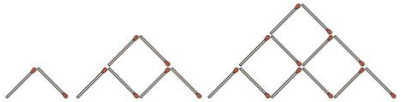
\includegraphics[scale=.6]{matches.png}
    \end{center}
  \end{minipage}
  \begin{enumerate}
      \item Déterminer les quatre premier termes de la suite.
      \item Exprimer $a_n$ en fonction de $n$ (avec $n\in\mathbb{N}^*$) puis en
        déduire la nature de la suite.
      \item Combien d'allumettes seront nécessaires pour construire la dixième
        étape ?
  \end{enumerate}
\end{exo}

\begin{exo}~\\
  \begin{minipage}[]{.5\textwidth}
    On construit des demi-disques comme sur la figure ci-dessous. L'unité est le
    centimètre. On appelle $a_n$ la longueur du demi-cercle correspondant au
    rang $n\geq1$.
    \begin{enumerate}
      \item Exprimer $a_n$ en fonction de $n$.
      \item Prouver que la suite $\left( a_n \right)$ est une suite arithmétique
        dont on déterminera la raison et le premier terme.
    \end{enumerate}
  \end{minipage}
  \begin{minipage}[]{.5\textwidth}
    \begin{center}
      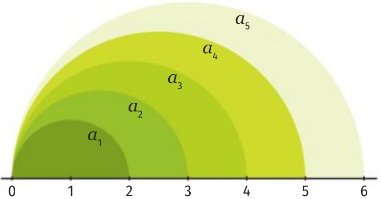
\includegraphics[scale=.6]{cercles.png}
    \end{center}
  \end{minipage}
  \begin{enumerate}
      \setcounter{enumi}{2}
      \item Pourra-t-on obtenir un demi-cercle dont la longueur sera supérieur à
        $25$ cm ? Si oui, à quelle étape ?
  \end{enumerate}
\end{exo}

\begin{exo}~\\[-10mm]
  \begin{minipage}[]{.5\textwidth}
    Dans le repère orthonormé ci-contre, on a représenté quelques termes de
    trois suites arithmétiques. Pour chacune de ces suites, répondre aux
    questions suivantes.
    \begin{enumerate}
      \item Déterminer le premier terme et la raison.
      \item Déterminer l'expression de $u_n$ en fonction de $n$.
      \item Donner les valeurs de $u_3$ et $u_6$.
    \end{enumerate}
  \end{minipage}
  \begin{minipage}[]{.5\textwidth}
    \begin{center}
      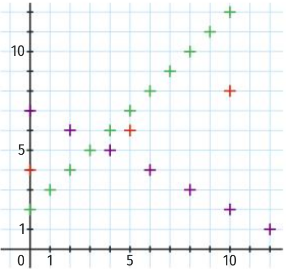
\includegraphics[scale=.7]{graph.png}
    \end{center}
  \end{minipage}
\end{exo}

\begin{exo}
  En 2017, le nombre d'abonnés à une page de réseau social d'une artiste était
  de $9000$. On suppose que, chaque année, elle obtient $1500$ abonnés
  supplémentaires. On note $f_n$ le nombre d'abonnés en $2017+n$ pour tout
  entier $n\in\mathbb{N}$.
  \begin{enumerate}
    \item Calculer le nombre d'abonnés en 2018 et 2019.
    \item Exprimer $f_{n+1}$ en fonction de $f_n$.
    \item Quelle est la nature de la suite ? En déduire une expression de $f_n$
      en fonction de $n$.
    \item Existe-t-il une année pour laquelle le nombre d'abonnés aura triplé
      par rapport à 2017 ? Si oui, laquelle ?
  \end{enumerate}
\end{exo}

\begin{exo}
  Fatima décide de s'entraîner pour une épreuve de natation, où elle devra nager
  sur une distance de $1500$ mètres. Pour cela, elle va dans une piscine dont la
  longueur est de $50$ m. Le premier jour, elle fait deux longueurs. Puis chaque
  jour, elle nage une longueur de plus que le jour précédent. On note $p_n$ la
  distance réalisée en mètres le $n$-ième jour.
  \begin{enumerate}
    \item Donner la valeur de $u_0$.
    \item Justifier que la suite $(u_n)$ est une suite arithmétique et
      déterminer sa raison.
    \item Au bout de combien de jours nagera-t-elle $1500$ m ?
  \end{enumerate}
\end{exo}

\begin{exo}
  Soit la suite $u$ définie sur $\mathbb{N}$ par $u_0=1$ et, pour tout entier
  naturel $n$, par $u_{n+1} = \frac{u_n}{2u_n+1}$.
  \begin{enumerate}
    \item \begin{enumerate}
        \item Calculer les quatre premiers termes de la suite $u$.
        \item La suite $u$ est-elle arithmétique ?
      \end{enumerate}
    \item On appelle $v$ la suite définie sur $\mathbb{N}$ par
      $v_n=\frac{1}{u_n}$.
      \begin{enumerate}
        \item Démontrer que la suite $v$ est arithmétique. On précisera sa
          raison et son premier terme.
        \item En déduire l'expression de $v_n$, puis celle de $u_n$, en fonction
          de $n$.
      \end{enumerate}
  \end{enumerate}
\end{exo}

\begin{exo}
  Soit $\left( u_n \right)$ une suite définie sur $\mathbb{N}$ par $u_0=-1$ et
  $u_{n+1}=\sqrt{u_n^2+3}$.
  \begin{enumerate}
    \item Montrer que la suite définie sur $\mathbb{N}$ par $v_n = u_n^2$ est
      une suite arithmétique.
    \item Donner l'expression de $v_n$, puis celle de $u_n$, en fonction de $n$.
    \item Déterminer la plus petite valeur de $n$ telle que $u_n\geq50$.
  \end{enumerate}
\end{exo}

\begin{exo}
  Soit $\left( \alpha_n \right)$ la suite définie par $\alpha_0 = 3$ et pour
  tout $n\in\mathbb{N}$, $\alpha_{n+1}=4-\frac{4}{\alpha_n}$. Soit également
  $\left( \beta_n \right)$ la suite définie pour tout $n\in\mathbb{N}$ par
  $\beta_n = \frac{1}{\alpha_n-2}$. On admet que la suite $\left( \beta_n
  \right)$ est bien définie.
  \begin{enumerate}
    \item Montrer que la suite $\left( \beta_n \right)$ est arithmétique.
    \item Exprimer $\beta_n$, puis $\alpha_n$, en fonction de $n$.
  \end{enumerate}
\end{exo}

\begin{exo}
  Pour chacune des suites suivantes, calculer $u_{20}$.
  \begin{enumerate}
    \item La suite géométrique $\left( u_n \right)$ de raison $q=3$ et telle
      que $u_3=12$.
    \item La suite géométrique $\left( u_n \right)$ de raison $q=-2$ et telle
      que $u_{31}=32$.
    \item La suite géométrique $\left( u_n \right)$ définie par $u_0=-5$ et,
      pour tout $n\in\mathbb{N}$, $u_{n+1}=2u_n$.
    \item La suite géométrique $\left( u_n \right)$ définie par $u_1=2048$ et,
      pour tout $n\in\mathbb{N}$, $u_{n+1}=-\frac{1}{2}u_n$.
  \end{enumerate}
\end{exo}

\begin{exo}
  Déterminer si les suites suivantes sont géométriques. Si oui, donner le
  premier terme ainsi que la raison.
  \begin{align*}
    \textbf{a)}\;& \forall n\in\mathbb{N},\; u_n = \frac{4^n}{3^{n+1}} &
    \textbf{b)}\;& \forall n\in\mathbb{N},\; u_n = \left( -7 \right)^n \\
    \textbf{c)}\;& \forall n\in\mathbb{N},\; u_n = 5n+2^n &
    \textbf{d)}\;& \forall n\in\mathbb{N},\; u_n = \frac{1}{3^n}
  \end{align*}
\end{exo}

\begin{exo}
  Afin de greffer $10$ cm$^2$ de peau à une personne brûlée, on lui prélève $20$
  mm$^2$. La culture permet d'augmenter de $15$\% la surface de peau chaque
  jour. On se demande dans combien de temps pourra se faire la greffe de peau.
  \begin{enumerate}
    \item Calculer la surface les deuxième et troisième jours.
    \item Pour tout $n\in\mathbb{N}$, on note $u_n$ la surface de peau le jour
      $n$. Écrire une relation entre $u_{n+1}$ et $u_n$.
    \item Quelle est la nature de la suite $\left( u_n \right)$ ?
    \item Donner l'expression de $u_n$ en fonction de $n$.
    \item Répondre au problème posé.
  \end{enumerate}
\end{exo}

\begin{exo}
  Le $1^\text{er}$ Janvier $2023$, Olivier veut déposer $5\;000$ euros sur un
  compte en banque. Il a le choix entre $2$ propositions.
  \begin{enumerate}
    \item On lui propose un compte épargne avec des intérêts à taux fixe. Chaque
      année, le $31$ Décembre, la banque lui verse $110$ euros sur son compte
      épargne. On note $u_n$ la somme sur le compte le $1^\text{er}$ Janvier de
      l'année $2023+n$.
      \begin{enumerate}
        \item Déterminer les valeurs de $u_0$ et $u_1$.
        \item Exprimer $u_n$ en fonction de $n$. Justifier.
        \item Combien aurait-il sur son compte en banque en $2040$ ?
      \end{enumerate}
    \item On lui propose un compte épargne avec des intérêts à taux composés.
      Chaque année, le $31$ Décembre, la banque lui verse sur son compte épagne
      $3$\% de la somme disponible sur le compte. On note $v_n$ la somme sur le
      compte le $1^\text{er}$ Janvier de l'année $2023+n$.
      \begin{enumerate}
        \item Déterminer les valeurs de $v_0$ et $v_1$.
        \item Exprimer $v_n$ en fonction de $n$. Justifier.
        \item Combien aurait-il sur son compte en banque en $2045$ ?
      \end{enumerate}
    \item S'il décide de laisser l'argent sur son compte pendant $5$ ans, quelle
      offre est la plus intéressante ?
    \item À l'aide de la calculatrice, déterminer à partir de combien d'années
      il est plus intéressant de choisir l'offre avec des intérêts à taux
      composés.
  \end{enumerate}
\end{exo}

\begin{exo}
  Soit $(u_n)$ la suite définie par $u_0=2$ et, pour tout $n\in\mathbb{N}$,
  $u_{n+1}=3u_n+4$.
  \begin{enumerate}
    \item Calculer $u_1$ et $u_2$.
    \item La suite $\left( u_n \right)$ est-elle arithmétique ? Géométrique ?
      Justifier.
    \item Soit $\left( v_n \right)$ la suite définie par pour tout
      $n\in\mathbb{N}$ par $v_n=u_n+2$.
      \begin{enumerate}
        \item Calculer $v_0$.
        \item Démontrer que $\left( v_n \right)$ est une suite géométrique de
          raison $3$.
        \item En déduire l'expression de $v_n$ en fonction de $n$.
        \item En déduire l'expression de $u_n$ en fonction de $n$.
      \end{enumerate}
  \end{enumerate}
\end{exo}

\begin{exo}
  Un parc d'attractions propose à ses visiteurs des pass annuels donannt un
  accès illimité à l'ensemble du site. En $2023$, $5\;000$ visiteurs achètent ce
  pass. Chaque année, le directeur du parc prévoit que $90$\% de ces visiteurs
  renouvelleront leur pass et que $800$ nouveaux visiteurs en achèteront un. On
  note $u_n$ le nombre de visiteurs ayant le pass annuel en $2023+n$.
  \begin{enumerate}
    \item Déterminer la valeur de $u_0$ et $u_1$.
    \item Justifier que, pour tout $n\in\mathbb{N}$, $u_{n+1} = 0,9u_n+800$.
    \item Soit $\left( v_n \right)$ la suite définie par $v_n=u_n-8000$.
      \begin{enumerate}
        \item Justifier que la suite $\left( v_n \right)$ est géométrique.
        \item Donner l'expression de $v_n$ en fonction de $n$.
        \item Donner l'expression de $u_n$ en fonction de $n$.
      \end{enumerate}
    \item Combien peut-on prévoir qu'il y aura de visiteurs détenteurs du pass
      annuel en $2035$ ?
  \end{enumerate}
\end{exo}

\begin{exo}
  On administre à un patient un médicament par injection intraveineuse. Le but
  de l'exercice est d'étudier l'évolution de cette quantité minute par minute.
  On programme la machine de façon que :
  \begin{itemize}
    \item à l'instant $0$, elle injecte $10$ mL de médicament ;
    \item toutes les minutes, elle injecte $1$ mL de médicament.
  \end{itemize}
  On estime que $20$\% du médicament présent dans le sang est éliminé par
  minute. On note $w_n$ la quantité de médicament (en mL) dans le sang après $n$
  minutes.
  \begin{enumerate}
    \item Justifier que pour tout entier naturel $n\in\mathbb{N}$, $w_{n+1} =
      0,8w_n+1$.
    \item Pour tout entier naturel $n\in\mathbb{N}$, on pose $z_n=w_n-5$.
      Démontrer que $z$ est une suite géométrique dont on précisera la raison et
      le premier terme.
    \item En déduire l'expression de $z_n$ puis de $w_n$ en fonction de $n$.
    \item Quelle est la limite de la suite $\left( w_n \right)$ ? Quelle
      interprétation peut-on donner ?
  \end{enumerate}
\end{exo}

\end{document}
